\documentclass{article}
\usepackage[utf8]{inputenc}
\usepackage{amsmath}
\usepackage{amsthm}
\usepackage{amssymb}
\newtheorem{theorem}{Theorem}[section]
\newtheorem{corollary}{Corollary}[theorem]
\newtheorem{lemma}[theorem]{Lemma}

\usepackage[colorlinks=true]{hyperref}
\usepackage[linesnumbered,algoruled,boxed,lined]{algorithm2e}
\usepackage{graphicx}
\usepackage{caption}
\usepackage{float}
\usepackage{multirow}
\usepackage{placeins}
\usepackage{hhline}
\usepackage{MnSymbol}

\def\d{\,{\rm d}}               % differential
\def\vc#1{\mathbf{\boldsymbol{#1}}}     % vector
\def\tn#1{\boldsymbol{#1}}
\def\eps{\varepsilon}
\def \E{{\mathsf E}}
\def \D{{{\rm I\kern-.3em D}}}
\newcommand{\norm}[1]{\left\lVert#1\right\rVert}
\def\prtl{\partial}
\def\todo#1{{\color{red}TODO: #1}}
\def\R{\mathbf{R}}
\def\pluseq{\mathrel{+}=}
\def\argdot{{\hspace{0.18em}\cdot\hspace{0.18em}}}
\def\Bavg#1{\Left\langle#1\Right\rangle}
\def\avg#1{\langle#1\rangle}
\def\var#1{\llangle#1\rrangle}
\def\Var{\mathop{\rm Var}}
\def\Cov{\mathop{\rm Cov}}
%\def\log{\mathop{\rm log}}
\def\abs#1{|#1|}
\DeclareMathOperator{\Span}{span}

\def\tvl{\vc{\tilde\lambda}}
\def\vl{{\vc\lambda}}
\def\estvl{{\vc{\hat\lambda}}}
\def\estrho{\hat\rho}
\def\vmu{\vc\mu}
\def\estvmu{{\vc{\hat\mu}}}
\def\vphi{\vc\phi}


\title{Robust Density Estimation Using Maximal Entropy Multilevel Monte Carlo method. }
\author{jan.brezina }
\date{September 2018}


\begin{document}

\maketitle

\section{Introduction}
Long term safety of an underground radioactive waste repository is assured primarily by the dilution and 
very slow transport of the contaminants through the suitable rock formations. Maximal concentrations of the contaminant on the surface is of major concern. Unfortunately reliable prediction of the surface concentration is not tractable due to lack of data about highly heterogeneous rock environment. In order to deal with these uncertainties we can model unknown rock properties as random fields and predict probability density function of the surface density. 
Classical Monte Carlo method needs at least several thousands of samples, which is prohibitively costly in the case of complex simulations. The Multilevel Monte Carlo (MLMC) method introduced by Giles \cite{Giles2008}, \cite{Giles2015} provides a way to estimate mean of an observable at the cost comparable to few forward simulations. Basic idea is to do high volume of samples using a less accurate but cheap approximation and much fewer samples of the difference between the observable and its approximation. If the difference have much smaller variance we obtain the mean estimate with same accuracy at fraction of cost.  The MLMC method has been already studied and analyzed in connection with variety of PDE problems: elliptic equations \cite{Barth2011a}, \cite{Cliffe2011a}, \cite{Abdulle2013}, parabolic equations \cite{Barth2013},
multiphase flow \cite{Muller2013}, \cite{Lu2016} and other.


Maximal entropy:
\cite{Barron1991}, \cite{Bierig2016a}

Elliptic eq. with log normal coefficients \cite{Graham2015}






 However the limitation is that MLMC can compute only approximation of expectation of any random variable. Therefore it is straight forward to make approximation of the mean, the variance and other moments, while it is not possible to approximate the quantiles and the distribution function directly. On the other way, the moment function or characteristic function are given in terms of expectations, which motivates a general approximation of the density function in terms of generalized moments.

Possible outcomes:
\begin{itemize}
    \item Research for suitable statistical models for complex hydrology problems (porosity, conductivity, dispersion, fracture openning, fracture density, ... dependency on the length scale).
    \item Demonstrate efficiency of MLMC for estimation various moments of relevant quantities of interest.
    \item Demonstrate efficient generation of samples for various types of correlations.
    \item Demonstrate reconstruction of the density function.
\end{itemize}

\section{Multilevel Monte Carlo method}
In this section we shall introduce the MLMC estimator and consider its application to a random variable based on a solution to a PDE.
Let $(\Omega, \Sigma, P)$ be a probability space and $X(\omega)$ be a random variable
which can not be sampled exactly, but we are able to sample its approximation $X^h(\omega)$. 
Consider classical MC approximation of the expectation $\E X$ by the sample mean:
\[
    \avg{X}_N = \avg{X^h}_N = \frac{1}{N}\sum_{i=1}^{N} X^h(\omega_i).
\]
As the estimator is unbiased, the mean square error (MSE) can be decomposed as:
\begin{equation}
    \label{eq:mc_mse}
    \E[\avg{X}_N - \E X]^2 = \E[\avg{X}_N - \E X^h ]^2 + \abs{\E X^h - \E X}^2
\end{equation}
The second term is error of the approximation $X^h$, which we assume to be sufficiently small further on.
The first term on the right hand side is the sampling error or the variance of the estimator:
\[
    \Var(\avg{X}_N) = \E[\avg{X}_N - \E X^h ]^2 = \frac{1}{N}\Var(X^h).
\]
 Classical MC method diminish the sampling error just by increasing $N$. Idea of the MLMC method is to introduce another approximation $X^H$ that is cheaper to sample and use the composed estimator
\[
	\E X^h \approx \avg{X}_{M,N} = \avg{X^H}_M	 + \avg{X^h - X^H}_N. 
\]
the estimator is unbiased with variance
\[
	\Var(\avg{X}_{M,N}) =  \frac{1}{M}\Var{X^H} + \frac{1}{N}\Var[X^h-X^H]. 
\]
Now we can increase the precision of the estimator by increasing the number $M$ of the cheap coarse samples, while keeping the number $N$ of the expensive fine samples low provided the variance
$\Var[X^h-X^H]$ is small. 

This aproach can be futher extened using a sequence of approximations $X^l = X^{h_l}$, for $l=1,\dots, L$.
Setting $X^0 = 0$ for the sake of consistency,
we obtain the MLMC estimator of $\E X$ in the form
\begin{equation}
    \label{eq:mlmc_est}
	\avg{X^L}_{\vc N} = \sum_{l=1}^L \avg{X^l - X^{l-1}}_{N_l} = \sum_{l=1}^L \avg{\Delta^l X}_{N_l}
\end{equation}
where $\vc N=(n_1,\dots, n_L)$ is the \emph{sampling vector} of the number of samples on individual levels 
and by $\Delta^l X(\omega) = X^l(\omega) - X^{l-1}(\omega)$ we denote level differences. Note that 
individual samples of the level differences must be based on the same realization $\omega$. 
Variance of the MLMC estimator is:
\begin{equation}
    \label{eq:var_mlmc}
    \Var( \avg{X^L}_{\vc N}) = \sum_{l=1}^L \frac{V_l}{N_l},\quad V_l = \Var(\avg{\Delta^l X}_{N_l}).
\end{equation}
The level variances $V_l$ can be estimated using the standard unbiased estimator:
\[
  V_l \approx \widehat{V}_l  = \frac{1}{N_l-1} \sum_{i=1}^{N_l} \big(\Delta^l X_i - \avg{\Delta^l X}_{N_l}\big)^2
\]


\subsection{Aplication to finite element solutions}
\todo{Very preliminary, make it more precise. Refer to other applied papers.}
In particular we are interested in the case $X=F(u)$, where $F$ is a functional representing an observation of
the solution $u$ to a PDE with some random data $d(\omega)$. The approximation $X^l = F(u^{h_l})$, $l=0,\dots,L$ is the same observation performed for an approximate solution $u^{h_l}$ computed on a mesh with the maximal element size $h_l$. Further on we assume $h_l = 2^{-\alpha l}$. Let $u$ be from a suitable space 
$W^* \subset W$, $u_h$ from $W_{h_l} \subset W$ and assume the usual error estimate in the form:
\[
	\norm{u - u_h}_{W} \le h^s \norm{u}_{W^*}
\] 
for some $s\ge 1$. See e.g. \cite{Evans1998}.
If $F:W \to R$ is bounded, then for $h=h_l$, $H=h_{l-1}$, we have
\[
	\abs{X^l - X^{l-1}} = \abs{F(u^h) - F(u^H)} \le \norm{F}\norm{u^h - u^H}_W \le C H^s\norm{u}_{W^*}
\]
and therefore 
\begin{equation}
    \label{eq:level_var_pde_est}
    V_l =  \E[X^l - X^{l-1}]^2 = C_u 2^{-\beta l},\quad \beta = 2s\alpha.
\end{equation}
By the same token we have 
\begin{equation}
    \label{eq:aprox_pde_est}
    \abs{\E X - \E X^L}^2 = C_u 2^{-2s\alpha L}
\end{equation}
Evaluation cost $C_l$ of the single sample difference $X^{l-1}(\omega) - X^l(\omega)$ is
\[
  C_l = \mathcal O( h_l^{-p}) \le C 2^{\gamma l}, \quad \gamma = p\alpha.
\]
For example in the case of linear elliptic equations using a multigrid solver one can get $p$ close to the problem dimension $d=1,2,3$. For more complex or time-dependent problems the power $p$ can be larger, but 
still it is usually independent of the choice of order of approximation $s$. Therefore, we may assume
$\beta > \gamma$. Applying \cite[Theorem 1]{Giles2015} for this case we conclude that for any target error 
$\epsilon< \frac{1}{e}$ we can found the sample vector $\vc N$ such that the MLMC estimator have the target error
\[
  \E[\avg{X}_N - \E X]^2 \le \epsilon^2
\]
and the total cost bounded as $C < c \epsilon^{-2}$.


\subsection{Optimal choice of number of samples}
Efficiency of the MLMC estimator \eqref{eq:mlmc_est} depends on the optimal choice of the sample vector $\vc N$. Basic analysis was done by Giles in \cite{Giles2008} and \cite{Giles2015}. In this section we report the formulas \eqref{eq:opt_n_for_var} and \eqref{eq:opt_n_for_cost} for optimal $\vc N$ in the case of given target variance $V$ or in the case of target cost $C$ respectively. Further, we propose slight modification suitable for practical usage.

Let  the level variances $V_l$ be given and let us denote $C_l$ the computational cost of a single sample of the difference $\Delta X^l$ at the level $l=1,\dots, L$. For a given target variance $V$ (c.f. \eqref{eq:var_mlmc}), we want to minimize the total cost
\begin{equation}
    \label{eq:total_cost}
	C = \sum_{l=1}^{L} C_l N_l.
\end{equation}
This leads to minimization problem for the functional
\[
	\Phi(N_1, \dots, N_L,\lambda) = \sum_l C_l N_l + \lambda \Big(\sum_l \frac{V_l}{N_l} - V\Big).
\]
Straightforward calculation then provides optimal choice of $\vc N$ for given $V$:
\begin{equation}
	\label{eq:opt_n_for_var}
	N_l^V = \sqrt{\frac{V_l}{C_l}} \frac{S}{V},\ \text{for }l=1,\dots, L,\quad \text{with } S = \sum_{i=1}^L \sqrt{V_i C_i}.
\end{equation}
Similarly we obtain $\vc N$ that minimize the total variance for the fixed total cost $C$ as
\begin{equation}
	\label{eq:opt_n_for_cost}
	N_l^C = \sqrt{\frac{V_l}{C_l}} \frac{C}{S}
	, \quad \text{for }l=1,\dots, L.
\end{equation}
Considering $V_l \le C_{v} 2^{-\beta l}$ and $C_l \le C_{c} 2^{\gamma l}$ we have total cost
\[
   C \le \frac{S^2}{V} = C_v C_c c \epsilon^{-2},
\]
where 
\[ 
   c = \left(\sum_{l=1}^{L} q^l\right)^2 \le (1-q)^{-2},\ q=2^\frac{\gamma - \beta}{2}
\]
for given target varaince $V=\epsilon^2$. Similarly, $V \le S^2 / C$ for given target cost $C$.



Formulas \eqref{eq:opt_n_for_var} and \eqref{eq:opt_n_for_cost} are based on the knowledge of the level variances $V_l$ and computational costs $C_l$ which are usually not known and must be estimated (see Section \ref{sec:VarEst}). These small errors lead to large changes in the optimal sample vector since related minimized functionals are quite flat at the optimal point.  This often results in overestimating the number of samples, especially on lower levels. To mitigate this problem we rather use
\[
	N_l^{V*} = \min( N_l^V, \frac{V_l L}{V} )
\]
for prescribed total variance $V$ and
\[
	N_l^{C*} = \min( N_l^C, \frac{C}{C_l L} )
\]
in the case of fixed cost $C$. This modification increase the total variance or total cost at most by $V$ and $C$ respectively, while keeping  $N_l$ reasonable. Indeed, let
\[
	N_l^{V*} = \frac{V_l L}{V} < N_l^V 
\]
happen for a single level $l$, then increase in the total variance is
\[
    V^* - V = \frac{V}{L} - \frac{V_l}{N_l^V} \le \frac{V}{L}
\]
and similarly for $N_l^{C*}$.



\subsection{Estimate level variances and costs}
\label{sec:VarEst}
As the exact values for $V_l$ and $C_l$ in \eqref{eq:opt_n_for_var} and \eqref{eq:opt_n_for_cost} are not available they are estimated from initial fraction of the samples. In particular $V_l$ is estimated by standard unbiased variance estimater $\widehat V_l$ and $C_l$ by a mean of times of collected samples 
$\widehat C_l$. Error of these estimates can be quite large especially on higher levels. 



In order to make MLMC algorithm fully automatic we have to estimate level variances $V_l$ from already collected samples. Since direct estimates are too inaccurate for higher levels we rather setup a regression model for $V_l$ and estimate its parameters using data from all levels. Moreover we also combine data for different moments.


Using the approximation:
\[
 \log \widehat V_l = \log V_l + \epsilon + O(\epsilon^2), \quad \epsilon = \frac{\widehat V_l - V_l}{V_l}
\]
we obtain approximation for its variance as:
\[
   \Var(\log \widehat V_l) = \Var\left[ \frac{\sum_{i=1}^{N_l} Y_i^2}{N_l -1}\right]  \approx \frac{1}{N-1}
\]
for some standardized i.i.d. samples $Y_i$.

Under assumption, that regression model $lm(\vc \alpha)$ fits well we have 
\[
 1 = (N-1) \Var[log \widehat V] = \E[ (\log \widehat V - lm(\alpha))^2 (N-1) ] 
\]


\[
  W_l = \sqrt{N_l-1}*(\log \widehat V_l - lm(\widehat{\vc\alpha}))
\]  
  is approximately $N(0,1)$. We use test for variance and possibly 
reduce number of levels used for regression. If
\[
  \sum_l W_l^2 > \chi^2_{N-1}(1-\alpha). 
\]
we reject hypothesis of the good fit.
\todo{Move variance approximation to notes since we need more testing}
Remarks:
\begin{itemize}
 \item Empirically, for the Flow problem, 9 level, for kvadratic model and using levels 3,4,5,6,7,8 for the fit we obtain variances that are significantly better then raw varainces.
 \item The hypothesis testing doesn't work. Even if it holds that $W_l$ is approximately $N(0,1)$.
 We obtain much higher values for the statistics. Further it depends on number of moments and number of used levels. 
 \item It behaves like it have much greater variance then 1, since $W_l^2$ values corresponds always to the p-values close to 1, which corresponds to big error of the fit.
 \item Questionable how it may work for smaller number of levels.
 \item Must also be tested for different simulations.
\end{itemize}




Let us assume that the level difference $Z_l^r = X_l^r - X^r_{l-l}$ for level $l=1,\dots L$ and a moment $r$ is normally distributed 
with mean estimate $\hat{Z}_l^r$ and variance estimate $V_l^r$ is
$$
W_l^r = \sum_{i} (Z^r_{l,i} - \hat{Z}_l^r)^2 / (n_l - 1).
$$

Where $Y_l = (n_l -1)W_l^r/V_l^r$ have distribution $\chi^2_{n_l -1}$.

We assume a simple model:
$$
  U_l^r = \log W_l^r =  \alpha_r + \beta \log h_l + \gamma (\log h_l)^2.
$$
where $h_l$ is a mesh step on level $l$ and $\alpha_r$, $\beta$ are parameters. 
For the variance of $U_l^r$ we have:
$$
  \D U_l^r = \D \log \Big( \frac{Y_l V_l^r}{n_l - 1} \Big) = \D \log (Y_l/N_l) = \epsilon_l
$$
with $N_l = n_l - 1$.

Then we estimate model parameters $\alpha_r$, $\beta$ from the least squares problem:
$$
    \tn{X}^T \tn{D}^2 \tn{X} \vc{b} = \tn{X}^T \tn{D} \vc{U},
    \ D_{i,i} = 1/\epsilon_{l}.
$$

Values of $\epsilon_l$ as a function of $l$ will be determined by MC. Note also that using the \href{https://en.wikipedia.org/wiki/Probability_density_function#Dependent_variables_and_change_of_variables}{Jacobi transform} we obtain PDF of $\epsilon_l$ as:
$$
    f(\epsilon) = \exp(\epsilon)N_l\chi^2_{n-1}(\exp(\epsilon)N_l).
$$
For small values of $N_l$ we compute $\D \epsilon_l$ using numerical quadrature. For sufficiently large $N_l$ we approximate $\chi^2$ by normal distribution:
$$
    f(\epsilon) = \exp(\epsilon)N_l\chi^2_{n-1}(\exp(\epsilon)N_l).
$$

\begin{figure}
 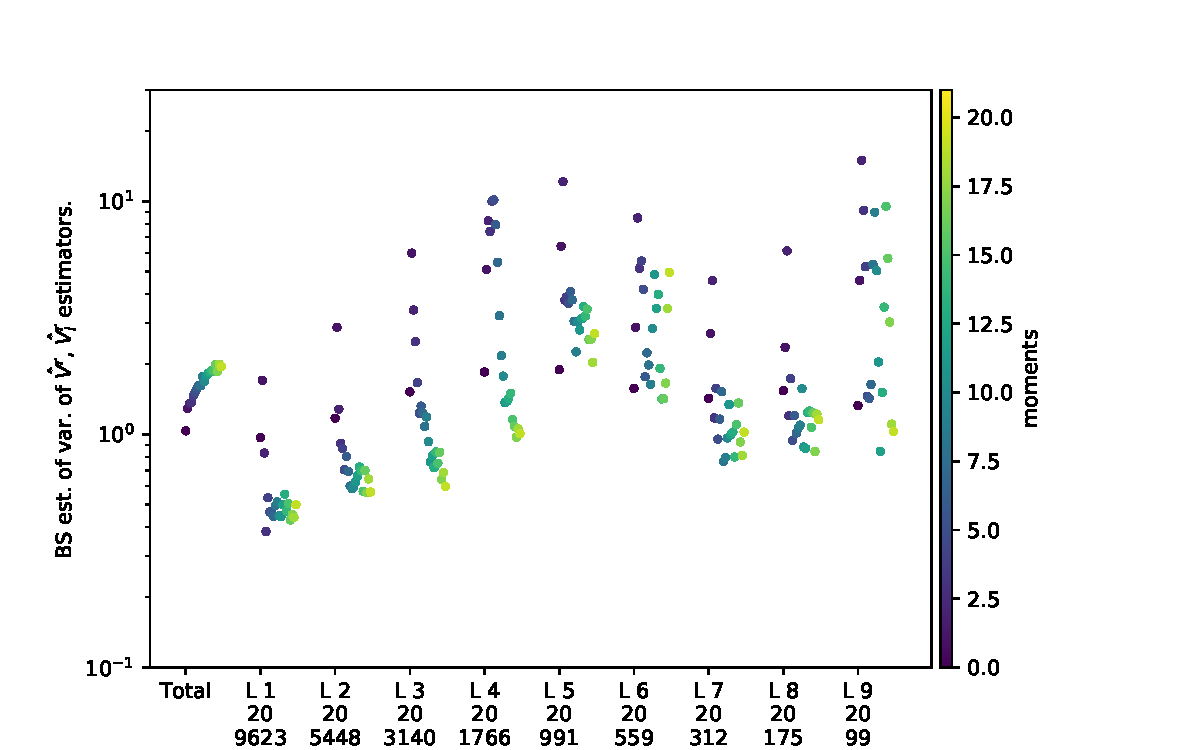
\includegraphics[width=0.55\textwidth]{bs_var_var_20.pdf}
 \hspace{-0.1\textwidth}
 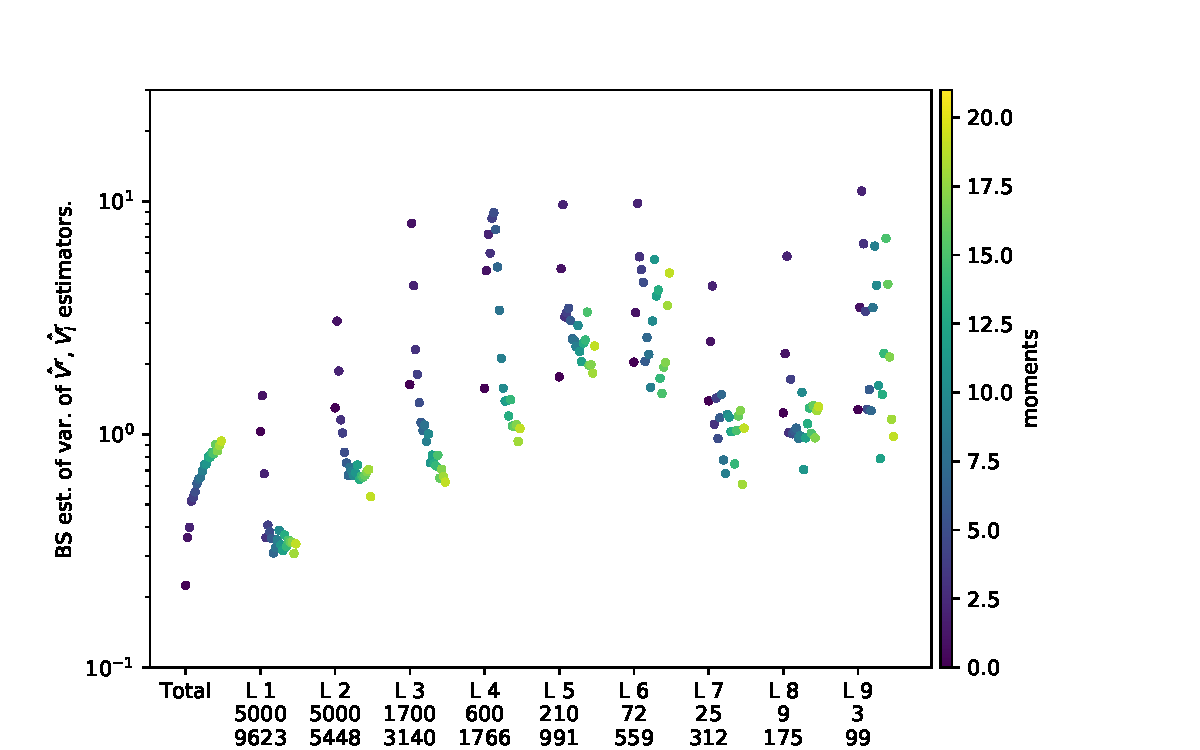
\includegraphics[width=0.55\textwidth]{bs_var_var_Nl.pdf}
 \caption{Estimate of error of estimators for $V^r$, $V_l^r$. Left figure demonstrate independece on level, right figure independence on $N_l$. Bootstrapping use 300 samples.}
 \label{fig:bs_var_var}
\end{figure}

\begin{figure}
 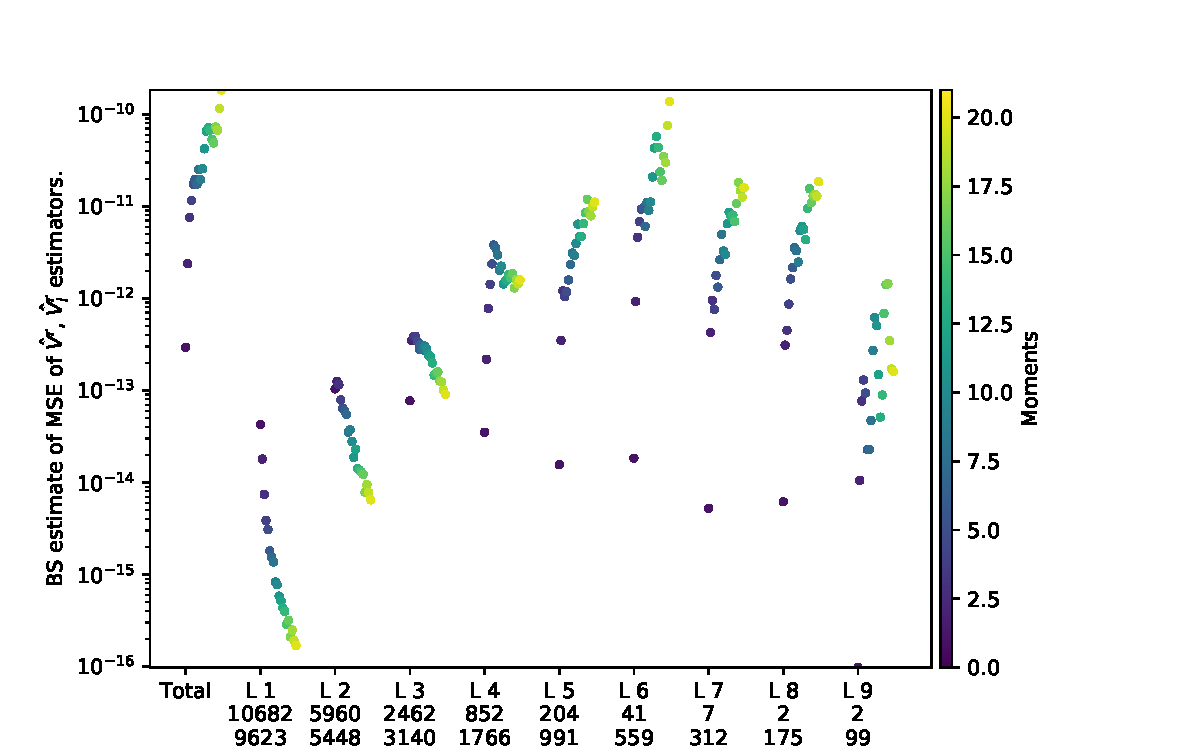
\includegraphics[width=0.55\textwidth]{bs_var_var_composition.pdf}
 \caption{BS estimate of the MSE of the variance estimate and its dropdown to individual levels. Realistic sample vector for a target variance $1e-4$.}
 \label{fig:bs_var_var_comp}
\end{figure}


\subsubsection{Uvahy}
Cilem je ziskat odhad rozptylu MLMC estimatoru, tak aby skutecny rozptyl byl mensi s danou pravdepodobnosti. 

Notes:
\begin{itemize}
    \item Variance $W_l$ of the level variance estimator is:
    \[
        Var \hat\sigma_l^2 \approx \hat\sigma_l^2 \frac{2}{N_l - 1}
    \]
    \dots assuming
    \[
    Z_l = \sum_{i=1}^{n_l}\Big(\frac{\Delta X^l_i}{\sigma_l}\Big)^2
    \]
    be approximately $\chi^2_k$ with $k=n_l$. This corresponds to the assumption that level differences $\Delta X_l$ have normal distribution. 
    \item At least for flow test case it seems that higher moments have smaller $W_l$ then first few (up to 10) moments. The differences in $W_l$ for individual moments are about one order of magnitude.  This effect is more pronounced for levels with many samples so it seems to be real. Differences between levels are also about one order of magnitude.
    \item These observations are not in contradiction with approximation of variance of  $\log W_l$.
\end{itemize}


\section{Maximal Entropy method}

The MLMC  estimator \eqref{eq:mlmc_est} can be applied to estimate any generalized moment $\E[\phi(X)]$ 
of the random variable $X$ using the same set of random samples. Taking a suitable 
set of such moments it is possible to construct an approximation to the PDF of $X$. This section first
summarize the Maximal Entropy method and related theoretical results slightly simplifying proofs form \cite{Barron1991}. Later we provide natural selection of the polynomial basis based on the estimate of the covariance matrix and we show that this choice significantly improves convergency of the related optimization problem.

Let $X$ be a continuous random variable with density function $\rho$ that have bounded support
$supp(\rho) \subset \Omega$ for a finite interval $\Omega \subset \R$. Further consider generalized moments
\begin{equation}
    \label{eq:gen_moments}
    \mu_m = \E_{\rho}[\phi_m(X)], \quad 
\end{equation}
for a finite set of linearly independent moment functions $\phi_1=1$, $\phi_m\in C^r(\Omega)$, $m=2,\dots, M$ forming a base of the space
\[
    \mathcal V_M = \Span\{\phi_m, m=1,\dots, M\}.
\] 
We shall use also the vector notation $\vphi = (\phi_1, \dots,\phi_M)$. The vector of moment values
$\vmu$ must be from $\mathcal M \subset \R^M$ with $\mu_1 = 1$.

Applying the MLMC estimator \eqref{eq:mlmc_est} and estimate of the variance \eqref{eq:var_mlmc} 
to the random variables $\phi_m(X)$, $m=1,\dots, M$ we obtain estimates of generalized moments
\begin{equation}
    \label{eq:mlmc_est_moments}
    \estvmu = \avg{\vphi} = \sum_{l=1}^L \frac{1}{N_l} \sum_{i=1}^{N_l} \Delta^l\vphi(X_i^l)
\end{equation}
as well as estimate for the error:
\[
    \Var(\avg{\vphi}_{\vc N}) =  \sum_{l=1}^{L} \frac{1}{N_l} \Var{\Delta^l\vphi} 
    \approx \sum_{l=1}^{L} \frac{1}{N_l} \var{\Delta^l\vphi}_{N_l}.
\]

Similarly, we can obtain MLMC estimate of the covariance matrix $\tn C = \Cov{\vc\phi}$: 
\begin{equation}
    \label{eq:mlmc_est_cov}
    \avg{\tn C} = \avg{(\vphi - \estvmu)\otimes(\vphi - \estvmu)}_{\vc N} = 
    \sum_{l=1}^L \frac{1}{N_l} \sum_{i=1}^{N_l} \Delta^l\Big[ 
    \big(\vphi(X_i^l) - \estvmu\big)\otimes\big(\vphi(X_i^l) - \estvmu\big)\Big].
\end{equation}
The same set of samples can be used in estimators \eqref{eq:mlmc_est}, \eqref{eq:mlmc_est_moments}, and \eqref{eq:mlmc_est_cov} as well as in the estimators of their errors.


Our next goal is to to find an approximation $\rho^M$ to the unknown density $\rho$ based only on values $\vmu \in \mathcal M$ of the generalized moments. From the infinte set of such densities we choose the one that maximize the Shanon's entropy,
$S = -\E_\rho[\log \rho]$,
which corresponds to the minimization of any additional information. 
In slight generalization of this approach, we assume a prior density $p$ and going to minimize the Kullbeck-Leibler divergence:
\[
    D(\rho\Vert p) = \int_\Omega \rho \log(\rho / p) \d x,
\]
under constrain $\E_\rho[ \vphi ] = \vmu$. 
% This leads to minimization of the functional:
% \begin{align}
%     \Phi(\rho, \vc\lambda) 
%     &= 
%     \int_\Omega \rho \Big( \vc\lambda \cdot \vc \phi - \log(\rho / p) \Big) \d x - \vc\lambda \cdot \vc\mu.
% \end{align}
Applying the Lagrange multipliers and taking variation with respect to $\rho$ the optimality conditions lead to the density in the form (se also \cite{...}):
\[
    \rho_{\vl}(x) = p e^{\vl\cdot\vphi}
\]
where we assume $\phi_1(x) = 1$ and $\mu_1 =1$. The parameters $\vl$ are solution
to the nonlinear system:
\begin{equation}
    \label{eq:moment_system}
    \vc G(\vl) = \int_\Omega \vphi\, p e^{\vl\cdot \vphi}\d x - \vmu = 0
\end{equation}
with the Jacobi matrix:
\[
    \tn H = \int_\Omega \vphi \otimes \vphi\, 
    p e^{\vl\cdot\vphi} \d x.
\]
\begin{lemma}
If $p$ is strictly positive and measurable on $\Omega$ and functions $\phi_m$,  $m=1,\dots,M$ are linearly independent, then matrix $\tn H$ is symmetric positive definite for any $\vl$.
\end{lemma}
\begin{proof}
For any non-zero $\vc u \in \R^M$ the function $f_{\vc u}(x) = \sum_m u_m \phi_m(x)$ is nonzero and thus
\[
    \vc u^T \tn H \vc u = \int_{\Omega} f_{\vc u}^2 p \exp\Big\{ \vc\lambda\cdot \vc\phi\Big\} \d x > 0.
\]
\end{proof}
The system \eqref{eq:moment_system} represents optimality conditions to the minimization problem
\begin{equation}
    \label{eq:min_problem}
    \text{minimize}(\vc\lambda):\quad F(\vl) = \int_{\Omega} \rho_{\lambda} - \vl\cdot\vmu.
\end{equation}
The functional is strictly convex due to strict convexity of $e^t$ (note also that $\tn H$ is SPD Hessian of $F$). 
Therefore the problem \eqref{eq:min_problem} posses a unique global minimum $\vl(\vmu)$ which is
also solution to the system \eqref{eq:moment_system}.


\subsection{Projection to exponential family}

Following \cite{Barron1991}, we can define set of densities with given moments $\vmu$:
\[
    C_{\vmu} = \{ \rho : \E_\rho[\vphi] = \vmu \}
\]
as well as the exponential family of densities:
\[
    \mathcal F_{p} = \{ \rho_\vl = 
    p e^{\vl\cdot\vphi} :
    \vl \in \Lambda\},\quad \Lambda = 
    \{\vl\in\R^M,\ \int_\Omega p e^{\vl\cdot\vphi} = 1\}.
\]
Then we can follow \cite[Lemma 2]{Barron1991} to get decomposition:
\begin{lemma}
\label{thm:decomposition}
For given $\vmu \in \mathcal M$ denote $\vl =\vl(\vmu)$ the unique solution to the system \eqref{eq:moment_system}. Then for any $\rho \in C_{\vmu}$ and $\estrho=\rho_\estvl \in\mathcal F_p$ the decomposition holds:
\begin{equation}
    \label{eq:decomposition}
    D(\rho\Vert\estrho) = D(\rho\Vert\rho_{\vl}) + D(\rho_{\vl}\Vert
    \estrho).
\end{equation}
In particular $\rho_{\vl}$ is minimizer of $D(\rho\Vert\rho_{\vl})$ over $\mathcal F_p$.
\end{lemma}
\begin{proof}
Due to \eqref{eq:moment_system} it holds $\E_{\rho}[\vphi] = \E_{\rho_{\vl}}[\vphi] = \vmu$. Then straightforward application of this identity yields:
\[
 D(\rho\Vert\estrho) = D(\rho\Vert\rho_{\vl}) 
 + \int_\Omega \rho (\vl - \estvl)\cdot \vc \phi = D(\rho\Vert\rho_{\vl}) + D(\rho_{\vl}\Vert\estrho).
\]
\end{proof}
The first term  on the right side of \eqref{eq:decomposition} corresponds to the approximation error of the familly $\mathcal F_p$ while the second term with $\estvl = \estvl(\estvmu)$ represents the error due to the moment estimation. 

\subsection{Approximation error}
Following estimates are based on \cite[Lemma 2]{Barron1991} 
\begin{lemma} 
  \begin{equation}
      \label{eq:l2_estimate}
      D(p\Vert q) \le \frac{1}{2}e^{\norm{\log p/q - c}_\infty} \norm{\log p/ q - c}_{L^2_p}^2
  \end{equation}

  
  \begin{equation}
      \label{eq:l1_estimate}
      D(p\Vert q) \le \frac{1}{2}\norm{\log p/ q}^2_{L^2_p} + \norm{\log p/ q}_{L^1_p}
  \end{equation}
 for any constant $c$.
\end{lemma}

Then for the approximation error we have:
\begin{lemma}
\label{thm:approx_error}
For given approximation space $\mathcal V_M$ and density $\rho\in C_{\vmu}$ let us denote
\[
  \epsilon = \epsilon_{M,\infty}(\rho) = \inf_{\vphi \in \mathcal V_M} \norm{\log \rho - \phi}_\infty.
\]
Then for the approximation error, we have estimate:
\[
D(\rho\Vert\rho_{\vl})  \le \frac{\abs{\Omega}}{2} e^{\epsilon} \epsilon^2.
\]
\end{lemma}
\todo{Jak je to s volbou $M$, z tohoto lematu by clovek rekl pokud zvolim dost vysoke $M$ tak mohu aproximovat libovolne presne a kovergence je rychla.
Na druhou z numerickych testu to vypada, ze pro vetsi $M$ dostavame velke oscilace v hustote. 
Jedno vysvetleni je, ze KL divergence muze byt mal i pro oscilujici aproximaci hustoty. Potrebujeme numericke testy pro presne hustoty.
Je nejaka sance udelat neco jako a posteriorni odhad?} 

\begin{proof}
Lemma \ref{thm:decomposition} states:
\[
D(\rho\Vert\rho_{\vl}) \le \inf_{\estvl \in \Lambda} D(\rho\Vert\rho_{\estvl})
\]
Now for any $\vc{\tilde\lambda} \in \R^M$, we can modify the first component to find $\estvl \in \Lambda$ satisfying
\[
  \estvl \cdot \vphi = \vc{\tilde\lambda} \cdot \vphi - \psi, \quad \psi 
                             = \log \int_\Omega p e^{\widetilde{\vc\lambda}\cdot \vc \phi}
\]
With such choice we have:
\[
D(\rho\Vert\rho_{\vl}) \le \inf_{\estvl \in \Lambda} D(\rho\Vert\rho_{\estvl})
=\inf_{\vc{\tilde\lambda} \in \R^M} D(\rho\Vert q_{\vc{\tilde\lambda}})
\]
Applying \eqref{eq:l2_estimate} with $c = \log p - \psi$, we obtain:
\[
  D(\rho\Vert q_{\vc{\tilde\lambda}}) \le 
  \frac{1}{2}
  e^{\norm{\log \rho - \vc{\tilde\lambda}\cdot \vc \phi}_\infty} 
    \norm{\log \rho - \vc{\tilde\lambda}\cdot \vc \phi}_{L^2_p}^2
  \le \frac{\abs{\Omega}}{2} e^{\epsilon} \epsilon^2.
\]
\end{proof}
For the case of polynomial approximation $\mathcal V_M = P^M(\Omega)$ we can directly apply results form \cite[Section 7]{Barron1991}. For a $\rho \in W^r_2(\Omega)$:
\[
    \epsilon_{m,\infty}(\rho) \le C \left(\frac{1}{m}\right)^{r-1} \norm{\rho}_{W^r_2},
\]
\[
    \epsilon_{m,2}(\rho) \le C \left(\frac{1}{m}\right)^{r}\norm{\rho}_{W^r_2}.
\]
\subsection{Estimation error}
We start with sensitivity estimate for the nonlinear system \eqref{eq:moment_system}.

\begin{lemma}
\label{thm:lambda_est}
Let $\estvl(\estvmu)$ be the solution of the system \eqref{eq:moment_system} for an approximation 
$\estvmu \in \mathcal M$ of the moments \eqref{eq:gen_moments} and let $\vl(\vmu)$ be the solution 
for exact moments $\vmu$. Then
\[
   \abs{\vl - \estvl} \le \frac{1}{\alpha_0} \abs{\vmu - \estvmu} 
\]
where $\alpha_0$ is the smallest eigenvalue of the Hessian matrix $\tn H(\estvl)$
\end{lemma}
\begin{proof}
Unfortunately we are yet unable to proof this result. So we try some numerical tests.

\includegraphics[width=\textwidth]{mu_to_lambda.pdf}

The blue dots have coordinates: $(|\vmu - \estvmu|, |\vl - \estvl|)$, blue lines are estimates for bounds from \cite{Barron1991}. The red dots are $(|\vmu - \estvmu|, \alpha_0|\vl - \estvl|)$,
red line have slope $\alpha_0$. The results for the six test distributions suggest validity of our estimate at least when the moment error $|\vmu - \estvmu|$ is not to large.

Further numerical tests confirms that the eigenvalues of the Hessian $\tn H(\estvl)$ are usually close to one. And smallest eigenvalue seems to increase as $\estvl$ tends to $\vl$. 
$\tn H(\estvl)$ should be very close to one, but it is not the case for some test distributions, but the limit value is somewhat smaller. Possibly that could be caused by insuficient normalization. 
However it seems that the lambda bound holds even without renormalization.

Here, we present some partial results and observations.
Let us denote $a=\vl\cdot\vphi$ and $b = \estvl\cdot\vphi$. We start with:
\[
  (\vl - \estvl)\cdot(\vmu - \estvmu)
      = \int_{\Omega} p \big[(\vl - \estvl)\cdot\vphi\big] (e^{(\vl\cdot\vphi} - e^{\estvl\cdot\vphi})
      =\int_{\Omega} p (a - b)(e^a - e^b)
\]

The next step is usage of $sinh$ expansion:
\[
 e^a - e^b = 2 e^{\frac{a+b}{2}}\frac{1}{2}\Big[e^{\frac{a-b}{2}} - e^{\frac{b-a}{2}}\Big] = 
 2 e^{\frac{a+b}{2}}\sinh(\frac{a-b}{2}),
\]
considering the expansion:
\[
    \sinh(x) = x + \frac{x^3}{6} + \frac{x^5}{120} + \dots
\]
we get an estimate
 \[
  (a-b)(e^a - e^b) \ge e^{\frac{a+b}{2}}\Big[|a-b|^2 + \frac{1}{24}|a-b|^4 + \dots\Big].
 \]

 All terms on the right have sign. Using just the first term, get a result:
\[
  (\vl - \estvl)\cdot(\vmu - \estvmu) \ge \int_{\Omega} p (a - b)^2(e^{a+b/2})
   \ge \frac{|\vl - \estvl|^2}{\alpha_0((\vl + \estvl)/2)}
\]
where $\alpha_0((\vl + \estvl)/2)$ is the smallest eigen value of the Hass matrix
$\tn H((\vl + \estvl)/2)$. This is not so good as we only know $\estvl$. 

 
 
 


% 
% The estimate starts with
% 
% Due to convexity of $f(t) = e^t$, we have
% \[
%     \frac{e^b - e^a}{b-a} \ge f'(\min(a,b))  = e^{\min(a,b)}
% \]
% for any $a, b\in \R$. Multiplying by $(b-a)^2\ge 0$ and using $\min(a,b) \ge a - |a-b|$, we get
% \begin{equation}
%   \label{eq:exp_ineq}
%   (b-a)(e^b - e^a) \ge e^a e^{-|a-b|}(b-a)^2 
% \end{equation}
%  
% 
% 
% Now we apply \eqref{eq:exp_ineq} with $a = \estvl\cdot\vphi$ and $b=\vl\cdot\vphi$ to estimate:
% \[
%   (\vl - \estvl)\cdot(\vmu - \estvmu)
%       = \int_{\Omega} p \big[(\vl - \estvl)\cdot\vphi\big] (e^{\vl\cdot\vphi} - e^{\estvl\cdot\vphi})
%       \ge \int_\Omega \big[(\vl - \estvl)\cdot\vphi\big]^2 pe^{\min(\estvl\cdot\vphi, \vl\cdot\vphi)}
% \]
% Further we can use:
% \[
%  \min(a, b) = \frac{a + b}{2} - \frac{|a - b|}{2}
% \]
% or 
% \[
%  \min(a, b) \ge a  - |a - b|.
% \]
% 
% Using $\sinh$:
% \[
%  e^a - e^b = 2 e^{\frac{a+b}{2}}\frac{1}{2}\Big[e^{\frac{a-b}{2}} - e^{\frac{b-a}{2}}\Big] = 
%  2 e^{\frac{a+b}{2}}\sinh(\frac{a-b}{2}),
% \]
% considering the expansion:
% \[
%     \sinh(x) = x + \frac{x^3}{6} + \frac{x^5}{120} + \dots
% \]
% 
%  
% Estimate according to Barron, Sheu \cite{Barron1991}. Lemma 5. 
% \[
%     |\vl_0 - \vl_r|^2 \le 2e^M e^\tau |\vl_0 - \vl_r| |\mu_0 - \mu_r|; \quad M = |\log  q/ \rho_0 |    
% \]
% 
%  
 
% We start our estimate with realization:
% \[
%     F_{\estvmu}(\vl_0) - F_{\estvmu}(\vl_r)  = -\mu_r(\vl_0 - \vl_r) \ge 0
% \]
% 
% \[
%     F_{\vmu}(\vl_r) - F_{\vmu}(\vl_0)  = -\mu_0(\vl_r - \vl_0) \ge 0
% \]

% \begin{align*}
%   (\mu_r - \mu_0) \cdot (\vl_r - \vl_0) &- \frac12 e^{-\tau} (\vl_0 - \vl_r) \tn H(\vl_r) (\vl_0 - \vl_r) \\
%   &=
%   \int_\Omega \Big[ e^{\vl_r\cdot\vphi} - e^{\vl_0\cdot\vphi} \Big] (\vl_r - \vl_0) \cdot \vphi 
%   -\int_\Omega  \frac12\big[ (\vl_0 - \vl_r) \cdot \vphi \big]^2 e^{\vl_r\cdot\vphi -\tau}\\
%   &\ge \frac12\int_\Omega  \big[ (\vl_0 - \vl_r) \cdot \vphi \big]^2 \big[e^\frac{(\vl_r + \vl_0) \cdot \vphi}{2} - e^{\vl_r\cdot\vphi-\tau}\big]
% \end{align*}

Applying this we get:
\[
  (\mu_r - \mu_0) \cdot (\vl_r - \vl_0) =
  \int_\Omega \Big[ e^{\vl_r\cdot\vphi} - e^{\vl_0\cdot\vphi} \Big] (\vl_r - \vl_0) \cdot \vphi 
  \ge \int_\Omega  \big[ (\vl_0 - \vl_r) \cdot \vphi \big]^2 e^\frac{(\vl_r + \vl_0) \cdot \vphi}{2}
\]
or more precisely:
\[
  (\mu_r - \mu_0) \cdot (\vl_r - \vl_0) =
  \int_\Omega  \big[ (\vl_0 - \vl_r) \cdot \vphi \big]^2 e^{\vl_r\cdot\vphi} e^\frac{(\vl_0 - \vl_r) \cdot \vphi}{2} S(x)
\]
where
\[
  S(x) = \sum_{n=0}^\infty \frac{|(\vl_0 - \vl_r) \cdot \vphi|^{2n}}{(2n+1)!2^{2n}}.
\]





Further we can estimate:
\[
    e^\frac{a + b}{2} \ge e^{a} - \abs{e^\frac{a + b}{2} - e^{a}}
\]
and then:
\[
 \abs{e^\frac{a + b}{2} - e^{a}} = 2e^\frac{3a+b}{4} \sinh\Big(\frac{|b-a|}{4}\Big)
\]

For any $0 \le x \le \tau$ we have $\sinh(x) \le \sinh(\tau) x$, thus
\[
 \abs{e^\frac{a + b}{2} - e^{a}} \le 2e^\frac{3a+b}{4} \sinh(\tau) \frac{|b-a|}{4}
 =  \sqrt{2\epsilon} e^{a/2}|a-b| \frac{\sinh(\tau)}{2\sqrt{2\epsilon}} e^{\frac{a+b}{4}}  \le 
    \epsilon e^{a}|a-b|^2 +  C e^{\frac{a+b}{2}}
\]
with $C = \frac{\sinh^2(\tau)}{16\epsilon}$.
combining together:
\begin{align*}
 (\mu_r - \mu_0) \cdot (\vl_r - \vl_0) 
 \ge (1-\epsilon)\int_\Omega  \big[ (\vl_0 - \vl_r) \cdot \vphi \big]^2 e^{\vl_r \cdot \vphi}
 -C \int_\Omega e^\frac{(\vl_r + \vl_0) \cdot \vphi}{2}
\end{align*}
However the last term is 











\[
 e^\frac{(\vl_r + \vl_0) \cdot \vphi}{2} - e^{\vl_r\cdot\vphi-\tau} \ge 
\]





\begin{align*}
  \alpha_0 e^\abs{\vl - \estvl}^2 &\le  (\vl-\estvl)^T\tn H(\estvl)(\vl -\estvl)\\
  &= \int_\Omega (\vl\cdot\vphi  - \estvl\cdot\vphi)^2 pe^{\estvl\cdot\vphi}
  \le \int_{\Omega} (\vl\cdot\vphi - \estvl\cdot\vphi) 
  p(e^{\vl\cdot\vphi} - e^{\estvl\cdot\vphi})\\
  &=  (\vl - \estvl)\cdot(\vmu - \estvmu) \le \abs{\vl - \estvl}\abs{\vmu - \estvmu}
\end{align*}
\end{proof}




Then for the estimation error we have following result.
\begin{lemma}
  \label{thm:est_error}
  Let $\rho_\lambda \in \mathcal F_p \cap C_{\vmu}$ for a $\vmu \in \mathcal M$, 
  and $\estrho = \rho_{\estvl}\in \mathcal F_p$ 
  where $\estvl$ is solution of \eqref{eq:moment_system} for $\estvmu \in \mathcal M$. Then 
  \[
    D(\rho_{\vl}\Vert \estrho) \le \frac{1}{\alpha_0} \abs{\vmu - \estvmu}^2
  \]
\end{lemma}

\begin{proof}
For any $\tvl$, we denote (c.f. \eqref{eq:min_problem}):
\[
F_{\estvmu}(\tvl) = \int_{\Omega} \rho_{\tvl} - \tvl\cdot\estvmu.
\]
In particular for $\vl$ that is solution of \eqref{eq:moment_system} with $\mu_1 = 1$, we have:
$F_{\estvmu}(\vl) = 1 - \vl\cdot\estvmu$. Similarly for $\estvl$ holds
$F_{\estvmu}(\estvl) = 1 - \estvl\cdot\estvmu$. Moreover, since $\estvl$ is minimizer 
of $F_{\estvmu}$, we conclude:
\[
 0\le F_{\estvmu}(\vl) - F_{\estvmu}(\estvl) = - \estvmu\cdot(\vl - \estvl).
\]
Now we can rewrite the KL-divergence as:
\[
  D(\rho_{\vl}\Vert \estrho) = (\vl - \estvl)\cdot \vmu \le
  (\vl - \estvl)\cdot (\vmu - \estvmu)
\]
Finally applying Lemma \ref{thm:lambda_est}
\[
D(\rho_{\vl}\Vert \estrho) \le \frac{1}{\alpha_0} \abs{\mu - \mu^*}^2
\]
 
\end{proof}
Similarly as in \cite[Theorem 3]{Barron1991} we  
\begin{theorem}
  \label{eq:estimate_err_var}
  Let $\rho_{\vl} \in \mathcal F_p \cap C_{\vmu}$ be the projection of the exact density $\rho$ to the exponential family based on exact moments  $\vmu = \E_\rho \vphi$. The MLMC estimator \eqref{eq:mlmc_est_moments} provides estimated moments $\estvmu$, we denote $\estrho = \rho_{\estvl}\in \mathcal F_p$ corresponding density with parameters $\estvl$ given by \eqref{eq:moment_system}.
  Assuming knowledge of the error $V = \E_{\rho} |\vmu - \estvmu|^2$, then for given (small) probability $\pi$
  we have
  \[
      P_{\rho}\Big( D(\rho_{\lambda}\Vert \estrho) \le \eta\Big) \ge 1 - \pi,\quad 
      \text{with } \eta = \frac{V}{\alpha_0 \pi},
  \]
  where $\alpha_0$ is the smallest eigenvalue of the Hessian matrix $\tn H(\estvl)$.
  
\end{theorem}
\begin{proof}
  Using Lemma \ref{thm:est_error} and applying Markov's inequality unbiased estimate $\estvmu$ we have:
  \[
   P\Big( D(\rho_{\lambda}\Vert \estrho) \ge \eta\Big) 
   \le P\Big( \abs{\vmu - \estvmu}^2 \ge \alpha_0  \eta\Big)
   \le \frac{\E_{\rho} |\vmu - \estvmu|^2}{\alpha_0 \eta} = \pi
  \]
\end{proof}


\todo{TODO:}

Cite estimates for $D(\rho\Vert\rho_{\lambda})$.

Modify estimates for $D(\rho\Vert\rho_{\lambda})$ using $q=p$ and
approximation of $Cov_p \vc phi$ for Legendere polynoms $\vc\phi$.

Probabilistic result $D(\rho_{\lambda*} \Vert \rho_{\lambda}) < V/p$
with probability at least $1-p$, where 
\[
    V = \sum_r \sum_l \frac{1}{N_l} \Var \delta^l\phi_r \approx \sum_r \sum_l \frac{1}{N_l} \hat{\Var} \delta^l\phi_r 
\]

\todo{Plot KL divergence between approximations for different $M$. We should have drop in error up to level where the Estimation error dominates.}
\todo{Choice of basis leading to $\alpha_0 \approx 1$.}

%%%%%%%%%%%%%%%%%%%%%%%%%%%%%%%%%%%%%%%%%%%%%%%%%%%%%%%%%%%%
\subsection{Nonlinear solver}

In this section we shall discus numerical solution of the minimization problem \eqref{eq:min_problem}. We prefere this setting over the direct solution of the nonlinear system \eqref{eq:moment_system} as it allows us to prescribe suitable regularization and penalization terms to improve the stability.
The problem is poorly conditioned unless we choose a basis in which $\tn H(\estvl)$ is close to identity matrix. Crucial observation is that $\tn H(\estvl)$ should be close to the non-centered 
covariance matrix of  $\vphi(X)$. In particular, if $\hat X$ is a random variable with PDF $\rho_{\estvl}$, then $\tn M \tn H(\estvl) \tn M^T = \Cov \vphi(\hat X)$, where 
\[
  \tn M = 
  \begin{pmatrix}
    -1    & 0 &\dots &0\\
    -\hat\mu_2    & 1 &\dots &0\\
    \vdots& 0 &\ddots      &\vdots\\
    -\hat\mu_n    & 0 &\dots &1
  \end{pmatrix}.
\]
Centering matrix $\tn M$ is so called \emph{involutory matrix}, i.e. $\tn M^{-1} = \tn M$.


Since $\rho_{\estvl}$ is approximation of $\rho$, the covariance of $\vphi(\hat X)$ should be close to the covariance of $\vphi(X)$ which can be estimated be the MLMC estimator \eqref{eq:mlmc_est_cov}.

In order to exploit these observations, we first choose an initial set of linearly independent 
moment functions $\phi_m$, $m=1,\dots,M$ with $\phi_1=1$. These form a base of the space $\mathcal V_M$.
Next, we compute the estimate $\hat{\tn C}$ of the covariance matrix using the estimator \eqref{eq:mlmc_est_cov}. The estimated matrix is still symmetric but need not to be positive definite
due to errors on individual levels of the MLMC estimator. 


Estimator gives non-central covariance estimate:
\[
 \avg{H}. 
\]
Then we compute the covariance approximation as: $\hat{\tn C} = \tn M \avg{H} \tn M^T$.
Then we compute eigenvalue decomposition $\hat{\tn C}= P \Lambda P^T$. 
Then we drop negative eigenvalues and in the remaining sequence
of decreasing values $\log \lambda_i$ we detect a construct a linear model for a floating window of eigenvalues and detect a point of rapid decrease of the values (Figure). Let us denote $N$ the number of remaining eigen values and eigenvectors. Having eigen values $\lambda_1 \dots \lambda_N$ and $M\times N$ matix $Q$ of remaining eigen vectors. It still holds $Q^T Q = I$ with $[N\times N]$. 
We have:
\[
   \tn H \approx M Q\Lambda' Q^TM^T
\]

We prescribe reduced set of momnet functions as:
\[
   \tilde\vphi = \tn R \tn L \vphi, \quad \tn L =  \tn R \Lambda^{-\frac12} Q^T \tn M
\]
for any ortonormal matrix $\tn R$. 
Now we have for $\hat{\tn H}$ ($N\times N$):
\begin{align*}
  \hat{\tn H} &= \E_{\estrho}\big[ \tilde\vphi \otimes \tilde\vphi\big] 
              = \tn L \E_{\estrho} \big[\vphi \otimes \vphi \big] \tn L^T 
              \approx \tn L \avg{\tn H} \tn L^T = \tn L \tn M \tn P \Lambda \tn P^T \tn M^T \tn L^T \\
              &\approx \tn L \tn M \tn Q \Lambda^{-\frac12} \Lambda^{-\frac12} \tn Q^T \tn M^T \tn L^T  = I 
\end{align*}


\todo{Ucesat}
\todo{Graf s poklesem vlastnich cisel}
\todo{Graf $\vphi$ for vlastni vektory.}



\section{Choice of moments}
\subsection{Monomials}
First choice for moment functions are monomials:
\[
    \phi_r(x) = x^r
\]
corresponding to classical moments.
In order to improve conditioning of the problem we should use centralized moments:
\begin{align}
    \phi_0(x) &= 1\\
    \phi_1(x) &= x - \mu_1\\
    \phi_r(x) &= \phi_r(x - \mu_1), \text{ for }r=1\dots R
\end{align}
with $\mu_0 = 1$.

However as the entropy function $e_n(x) = -\ln(\rho_n)$ is a linear combination of the generalized moment functions, it may expect that using monomials leads to badly conditioned non-linear problem. In order to 
get better conditioning needs to choice moment functions to be nearly orthogonal and possibly with small support.

\subsection{Fourier moment functions}


\subsection{Spline approximation}
In order to keep Jacobi matrix well conditioned can keep supports of $\phi_r$ to be mostly disjoint since if $supp \phi_r$ is disjoint with $supp \phi_s$ we have $H_{rs} = 0$.
In order to keep basic smoothness, we may use spline base functions, in particular cubic splines.



\section{Synthetic experiments}
\section{Correlated random fields}
We what to generate realizations of a random field: $Z(\vc x, \omega)$, for $\vc x$ in domain $D \subset R^d$. We consider {\it second order field}, i.e. with finite variance for every $\vc x\in D$. For such fields we can define mean:
\[
    \mu_Z(\vc x) = \E\big[ Z(\vc x) \big]
\]
and covariance:
\[
    C_Z(\vc x, \vc y) = \E\big[ (Z(\vc x) - \mu(\vc x))(Z(\vc y) - \mu(\vc y)) \big]
\]

We restrict ourself to the case of stationary fields, where $C$ depends only on $(\vc x - \vc y)$. Our aim is to compute lot of realizations of the field fro a fixed set of points. Further on, we focus on the zero-mean fields:
\[
    \tilde Z(\vc x) = Z(\vc x) - \mu(\vc x), \E(\tilde Z) = 0.
\]

TODO:
\begin{itemize}
\item Approximation of quantiles or distribution function via. density is not optimal, since the error is accumulated through integration of the density. Consider approximation of distribution via. approximation of Havyside function (see Giles), propose some approximation for quantiles.

\item Derive error estimates for density, quantiles, distribution  for various set of moments. How to approximate tails? Is the maximum entropy the best choice?

\item How to use MLMC for generated random fractures, in particular how to make two generated fracture sets that are "correleated".
\end{itemize}

\section{Numerical experiments}

\subsection{MLMC sampling algorithm}
Optimal choice of the sample vector $\vc N$ given by \eqref{eq:opt_n_for_var} or \eqref{eq:opt_n_for_cost} is function $N^{opt}(\vc V, \vc C)$ of the vector of level variances $\vc V$ and the vector of level costs $\vc C$. As $\vc V$ and $\vc C$ are not known a priori, we want to estimate them on the fly from the increasing set of collected samples. as we collect the samples.  Level variances $V_l$ are estimated by the regression \eqref{eq:regression}, sample cost $C_l$ is simply the average sample time of collected samples on the level $l$. 
In order to collect optimal number of samples we designed a simple iterative Algorithm \ref{algo_sampling}. 
Initial vector of scheduled samples $N^s_0$ is fixed, in particular we use an arithmetic sequence decreasing form $100$ to $0$. Vector $\vc N^t_0$ of target number of samples is set to $2\,\vc N^s_0$. The iteration $i$ starts with scheduling new samples up to the $\vc N^s_i$.
Then we wait until at least half of $N^s_i$ is computed. \todo{"half of samples is done" ... to je divne, neni jasne pulka kterych by to mela byt, a jestli to musi byt pulka.}. We collect computed samples and use all available samples to update estimates $\vc V_i$ and $\vc C_i$ for level variances and costs respectively.
Using these new estimates we determine new target sampling vector $\vc N^t_{i+1}$ and
add fraction $\alpha$ of the difference to $\vc N^t_{i}$. We iterate until relative difference between target and scheduled sampling vectors is greater then tolerance $\epsilon$ for any level $l$.
In practice we use parameters $\alpha=0.1$ and $\epsilon = 0.0$

\begin{algorithm}
    \SetAlgoLined
    \DontPrintSemicolon
    %
    $\vc N^s_0 \gets ( 100, ..., 3)$\;
    $\vc N^t_0 = 2 \vc N^s_0$\;
    $i \gets 0$\;
    \While{ $N^t_{i,l} - N^s_{i,l} > \eps N^s_{i,l}$ for any $l$ }{
        schedule new samples up to $\vc N^s_i$\;
        wait until half of samples is done\;
        estimate $\vc V_i$, $\vc C_i$ from collected samples\;
        $\vc N^t_{i+1} \gets N^{opt}(\vc V_i, \vc C_i)$\;
        $\vc N^s_{i+1} \gets \vc N^s_i + \alpha(\vc N^t_{i+1} - \vc N^s_i)$\;
        $i \gets i+1$\;
    }
    \label{algo_sampling}
    \caption{MLMC samples number estimation}
\end{algorithm}

Progress of the algorithm is depicted at Figure \ref{fig:n_l_time}.  ... 

\break
Following graph \ref{fig:n_l_time} and table \ref{mlmc_sampling} provide data for the task of water flowing through unit square using flow123d \cite{flow123d} software. We use five level MC method. Different meshes were created at different levels. First level mesh had just 6 elements, higher levels had meshes with 78, 1730, 40818 and 997606 elements. Whole task was performed on cluster that contains 20 nodes each of them has 2x 10-core CPU and 96 GB RAM, this allowed us to perform parallel computing of samples. Individual sample computations were grouped to the jobs that were scheduled in cluster by PBS software. Each job had approximately same computational cost. Cluster traffic affects the number of currently running jobs. As a result, it can affect the fluency of the sample computations. That probably caused jump $C^c$ around 40th iteration in \ref{fig:n_l_time}.

\todo{Popsat jake byly velikosti siti na jednotlivych urovnich a jaka to vubec byla uloha. Popsat zhruba HW na kterem to bezelo, a davkove zpracovani pomoci PBS. Okomentovat nerovnomerny prubeh krivky dokoncenych vzorku.}
\begin{figure}[H]
\centering
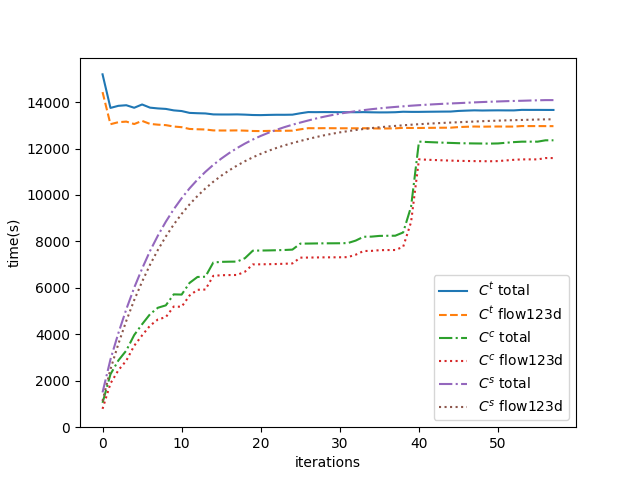
\includegraphics[width=\textwidth]{time_1.png}
\caption{Evolution of CPU time for target $C^t$, scheduled $C^s$ and collected samples during iterations of Algorithm \ref{algo_sampling}.}
\label{fig:n_l_time}
\end{figure}
\todo{Upravit typ car: barvou rozlisit $C^s$, $C^t$, $C^c$, plnou carou kompletni cas, carkovane pouze vypocet Flow123d. Tu carkovanou bych udelal jen pro $N_c$. Takze by tam nakonec byly 4 cary.}
V tomto grafu jsou $C^s$ - naplánované vzorky (estimated), $C^c$ jsou již dokončené vzorky (collected), $C^t$ jsou cílové vzorky pokud bychom je určovali z $C^c$. Po skončení celé MLMC by byly $C^c$ a $C^s$ stejné, $C^t$ jsou na konci menší než $C^s$, protože se ukazuje, že jsme na začátku napočítali více vzorků na nižších úrovních [17, 7, 3] a stačilo by [12, 2, 2]. Různý typ čar jsem zvolil kvůli tomu kdyby to nakonec bylo černobíle, tak aby to bylo k přečtení. Pokud by tam zůstali ty přidané křivky, tak už by to nešlo oddělit stylem čáry. 
\todo{Proc je graf nakonci uriznuty? Mozna tu tabulku uplne zrusime, ale do grafu by se tedy jeste hodil odhadovany cas naplanovanych uloh. To je asi ten cas estimated v tabulce.  Bylo by z toho snad videt, ze mame celou dobu previs naplanovanych uloh na provedenymi.}

\begin{table}[]
\caption{Sampling algorithm iterations}
\centering

\begin{tabular}{|l|l|l|l|l|l|l|}
\hline
iteration                                  & samples  & $l_{1}$     & $l_{2}$   & $l_{3}$  & $l_{4}$ & $l_{5}$ \\ \hhline{|=|=|=|=|=|=|=|}
{\multirow{2}{*}{0}} & collected & 100    & 41    & 17  & 7  & 2  \\ 
                   & estimated & 2204   & 402   & 17  & 7  & 3  \\ \hline
\multirow{2}{*}{1}                       & collected & 1112   & 402   & 17  & 7  & 3  \\  
                                         & estimated & 3955   & 612   & 17  & 7  & 3  \\ \hline
\multirow{2}{*}{2}                       & collected & 2103   & 432   & 17  & 7  & 3  \\  
                                         & estimated & 5545   & 801   & 17  & 7  & 3  \\ \hline
% \multirow{2}{*}{3}                       & collected & 2789   & 481   & 17  & 7  & 3  \\  
%                                          & estimated & 6982   & 971   & 17  & 7  & 3  \\ \hline
\multirow{2}{*}{4}                       & collected & 3777   & 654   & 17  & 7  & 3  \\  
                                         & estimated & 8261   & 1118  & 17  & 7  & 3  \\ \hline
% \multirow{2}{*}{5}                       & collected & 4455   & 785   & 17  & 7  & 3  \\ 
%                                          & estimated & 9435   & 1253  & 17  & 7  & 3  \\ \hline
\multirow{2}{*}{10}                      & collected & 6517   & 926   & 17  & 7  & 3  \\  
                                         & estimated & 12979  & 1642  & 17  & 7  & 3  \\ \hline
% \multirow{2}{*}{15}                      & collected & 8668   & 1216  & 17  & 7  & 3  \\  
%                                          & estimated & 15646  & 1920  & 17  & 7  & 3  \\ \hline
\multirow{2}{*}{20}                      & collected & 9457   & 1268  & 17  & 7  & 3  \\  
                                         & estimated & 17181  & 2078  & 17  & 7  & 3  \\ \hline
% \multirow{2}{*}{25}                      & collected & 9950   & 1287  & 17  & 7  & 3  \\ 
%                                          & estimated & 18081  & 2172  & 17  & 7  & 3  \\ \hline
\multirow{2}{*}{30}                      & collected & 9972   & 1293  & 17  & 7  & 3  \\  
                                         & estimated & 18671  & 2247  & 17  & 7  & 3  \\ \hline
% \multirow{2}{*}{35}                      & collected & 10488  & 1322  & 17  & 7  & 3  \\ \ 
%                                          & estimated & 19021  & 2292  & 17  & 7  & 3  \\ \hline
% \multirow{2}{*}{40}                      & collected & 16739  & 2102  & 17  & 7  & 3  \\  
%                                          & estimated & 19233  & 2317  & 17  & 7  & 3  \\ \hline
% \multirow{2}{*}{45}                      & collected & 16656  & 2065  & 17  & 7  & 3  \\  
%                                          & estimated & 19368  & 2334  & 17  & 7  & 3  \\ \hline
% \multirow{2}{*}{50}                      & collected & 16647  & 2055  & 17  & 7  & 3  \\  
%                                          & estimated & 19473  & 2355  & 17  & 7  & 3  \\ \hline
% \multirow{2}{*}{54}                      & collected & 16747  & 2050  & 17  & 7  & 3  \\  
%                                          & estimated & 19504  & 2361  & 17  & 7  & 3  \\ \hline
\multirow{2}{*}{55}                      & collected & 16782  & 2051  & 17  & 7  & 3  \\  
                                         & estimated & 19544  & 2370  & 17  & 7  & 3  \\ \hline
\multirow{2}{*}{56}                      & collected & 16783  & 2051  & 17  & 7 & 3  \\  
                                         & estimated & 19556  & 2373  & 17  & 7 & 3  \\ \hline
\end{tabular}
\end{table}
\FloatBarrier




\section{Sampling  of Random Fields}
This section is devoted to the problematic of generating cross-correlated random fields.

\subsection{Random Field}
Any scalar random field $u(\vc x)$ with mean field $\mu(\vc x)$ and standard error
field $\sigma(\vc x)$ can be normalized as:
\[
    u(\vc x) = \mu(\vc x) + \sigma(\vc x) \tilde{u}(\vc x)
\]
where $\tilde{u}$ is a \emph{normalized} random field with zero mean and variance equal to $1$. Therefore we shall discuss only generation of normalized random fields further on. The normalized random field is given by its correlation function:
\[
    {\rm Cov}(u(\vc x), u(\vc y) ) = c(\vc x, \vc y)  
    = \E\big[ (u(\vc x) - \E u(\vc x))(u(\vc y) - \E u(\vc y)) \big]
\]
The field is called \emph{stationary} if $c(\vc x, \vc y) = c(\vc x - \vc y)$, i.e. 
correlation function depends on direction vector but is invariant to changes in position. The field is called \emph{isotropic} if $c(\vc x, \vc y) = c(|\vc x - \vc y|)$, i.e. it is also invariant with respect to rotations. 

The Wiener-Kintchine theorem states that
\cite{}

\subsection{Variogram function}
Instead of correlation function we can use the \emph{variogram function} $\gamma$:
\[
    \gamma(u(\vc x), u(\vc y)) = \frac12 \E\big[u(\vc x) - u(\vc y)\big].
\]
General relation ship between $c$ and $\gamma$ is quite complicated, but if we assume $\E u(\vc x) = 0$, then
we have:
\[
    \gamma(\vc x, \vc y) = \frac12 \big[ c(\vc x, \vc x) + c(\vc y, \vc y)\big] - c(\vc x, \vc y)
\]
and in the case of normalized random field:
\[
    \gamma(\vc x, \vc y) = 1 - c(\vc x, \vc y)
\]


There are two kinds of methods: decomposition and spectral methods. The decomposition methods use singular value decomposition of the correlation matrix for a fixed set of evaluation points. And use incomplete factorization of the Karhunen-Lo\`eve expansion:
\[
    Z(\vc x, \omega) = \mu(\vc x) +  \sum_{i = 1}^\infty \sqrt{\lambda_i} \xi_i(\omega) \phi_i(\vc x)
\]
where  $\xi_i$ are uncorrelated random variables, $\lambda_i$ are the eigenvalues and  $\phi_i$ are 
the eigenfunctions of the correlation operator. In the case of fixed evaluation points we have just finite
dimension, correlation operator is correlation matrix and sum is finite. As the eigenvalues usually decrease
rapidly we can use truncated sum, i.e. truncated KL expansion.

The spectral methods sample the field by its Fourier Second kind of methods use sp

\section{Numerical experiments}
\begin{figure}
    \centering
    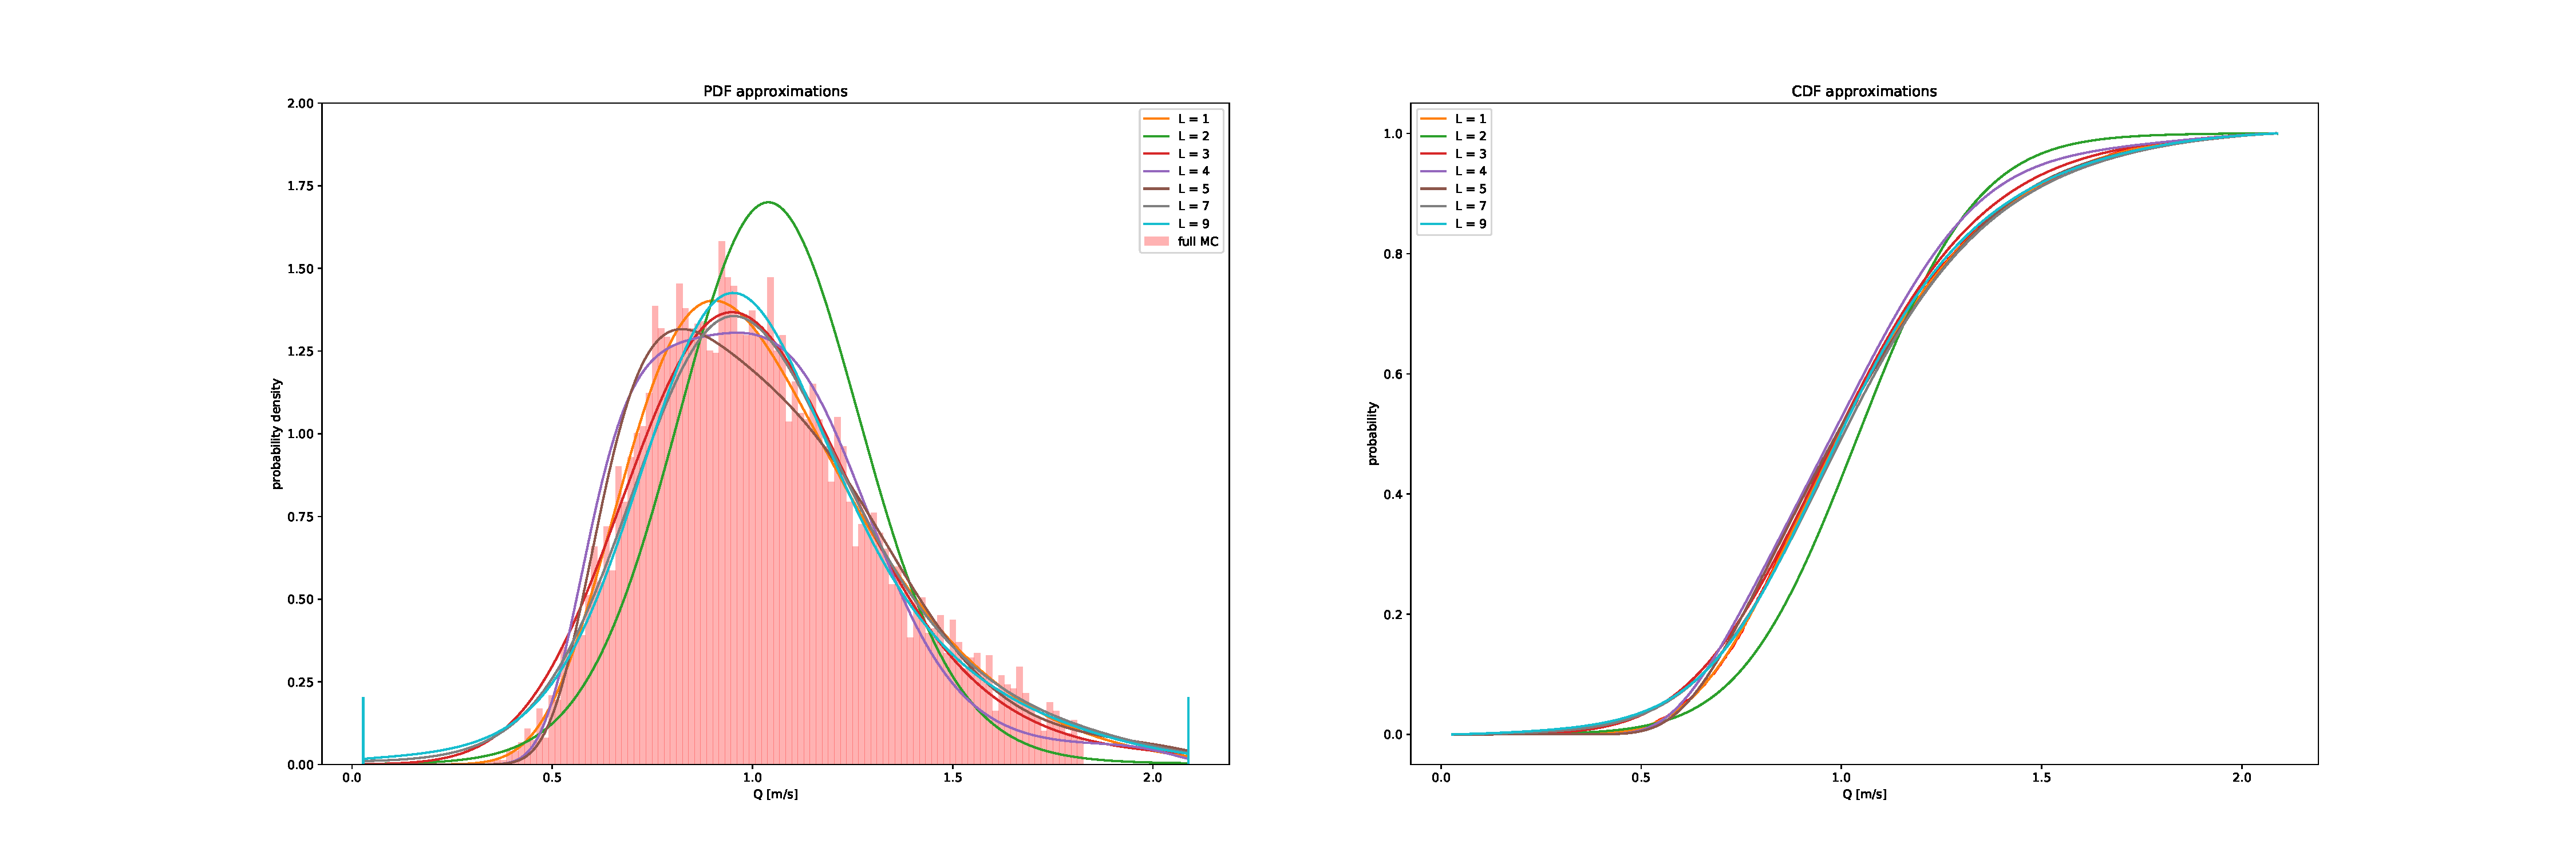
\includegraphics[width=\textwidth]{01_cond_pdf_cdf.pdf}
    \caption{Approximation a PDF of the total flux through a square domain with random conductivity. Use 11 Legendere moments.}
    \label{fig:flux_approx_pdf}
\end{figure}
\todo{Divne je, ze je ten histogram (a stejne tak vsechny histogramy prvnich urovni) uriznuty vpravo.}

\subsection{Model transport problem}
\section{Conclusions}



\bibliographystyle{plain}
\bibliography{theory.bib}








\end{document}

